\section{Grafer}
\subsection*{Begrep}
\begin{frame}
    \begin{block}{Graf $G(V,E)$}
    En Graf $G$ er en tuple med en set av noder $V$ og en set av kanter (edges) $E$
    \end{block}

\begin{columns}
    \begin{column}{0.28\textwidth}
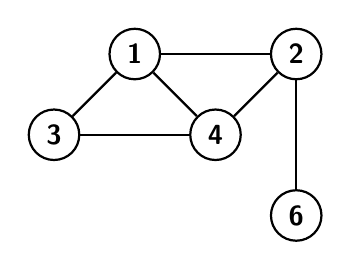
\begin{tikzpicture}[
    node distance=1.45cm, thick,
    main node/.style={circle, draw, font=\sffamily\bfseries}
]
    \node[main node] (1)                    {1};
    \node[main node] (3) [below left  of=1] {3};
    \node[main node] (4) [below right of=1] {4};
    \node[main node] (2) [above right of=4] {2};
    \node[main node] (6) [below right of=4] {6}; % <-4> forces an additional overlay in which node 2 disappears

    \path (1) edge (2)
        (4) edge (2)
        (6) edge (2);
    \path (1) edge (3)
        (4) edge (1);
    \path (3) edge (4);
\end{tikzpicture}
 \end{column}
    \begin{column}{0.68\textwidth}
\begin{itemize}
    \item<1-> Noder: $V={1,2,3,4,6}$
    \item<2-> Kanter: $E={(1,2), (1,4), (3,4), (2,4), (2,6), (1,3)}$
    \item<3-> Path: Vei fra A til B\\
    Eksempel: $Path(1,6)=(1,2,6)$
    \item<4-> Cycle: En path med samme start og slutt\\
    Eksempel: $(1,3,4,1)$, $(1,2,4,3,1)$
    \item<5-> Naboer: Set of noder som har en kante til en node\\
    Eksempel: $N(4)={1,2,3}$, $N(6)=2$
    \item<6-> Degree: Antall naboer av en node\\
    Eksempel: $deg(4)=3$, $deg(6)=1$
\end{itemize}
 \end{column}
\end{columns}
\end{frame}

\begin{frame}{}
    \begin{columns}
    \begin{column}{0.48\textwidth}
    \begin{figure}
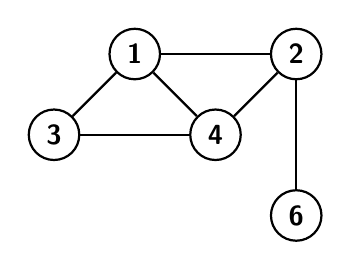
\begin{tikzpicture}[
    node distance=1.45cm, thick,
    main node/.style={circle, draw, font=\sffamily\bfseries}
]
    \node[main node] (1)                    {1};
    \node[main node] (3) [below left  of=1] {3};
    \node[main node] (4) [below right of=1] {4};
    \node[main node] (2) [above right of=4] {2};
    \node[main node] (6) [below right of=4] {6}; % <-4> forces an additional overlay in which node 2 disappears

    \path (1) edge (2)
        (4) edge (2)
        (6) edge (2);
    \path (1) edge (3)
        (4) edge (1);
    \path (3) edge (4);
\end{tikzpicture}
\caption{Urettet graf (undirected)}
\end{figure}
\begin{itemize}
    \item $deg(4) = 3$
\end{itemize}
 \end{column}
    \begin{column}{0.48\textwidth}
    \begin{figure}
    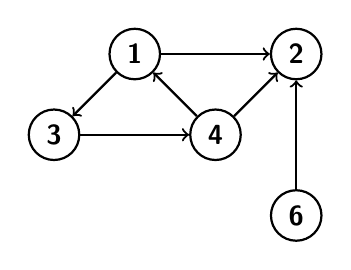
\begin{tikzpicture}[
    node distance=1.45cm, thick,
    main node/.style={circle, draw, font=\sffamily\bfseries}
]
    \node[main node] (1)                    {1};
    \node[main node] (3) [below left  of=1] {3};
    \node[main node] (4) [below right of=1] {4};
    \node[main node] (2) [above right of=4] {2};
    \node[main node] (6) [below right of=4] {6}; % <-4> forces an additional overlay in which node 2 disappears

    \path[->] (1) edge (2)
        (4) edge (2)
        (6) edge (2);
    \path[->] (1) edge (3)
        (4) edge (1);
    \path[->] (3) edge (4);
\end{tikzpicture}
\caption{Rettet graf (directed)}
\end{figure}
\begin{itemize}
    \item $deg^-(4) = 1$ (ingoing)
    \item $deg^+(4) = 2$ (outgoing)
\end{itemize}
 \end{column}
\end{columns}
\end{frame}

\begin{frame}
    \begin{block}{Bipartite graf $G(V,A,B)$}
    Set av nodene er delt i to sets $A,B$ der alle kanter $v\in V$ går fra en node i $A$ til en node i $B$\\
    Grafen kan farges i to farger med ingen to nabonoder i samme farge
    \end{block}

\begin{tikzpicture}[
    node distance=1.45cm, thick,
    main node/.style={circle, draw, font=\sffamily\bfseries}
]
    \node[main node,onslide=<2->{fill=black!40!green}] (1)                    {1};
    \node[main node,onslide=<2->{fill=black!40!green}] (3) [below left  of=1] {3};
    \node[main node,onslide=<2->{fill=black!40!green}] (4) [below right of=1] {4};
    \node[main node,onslide=<2->{fill=black!30!red}] (2) [above right of=4] {2};
    \node[main node,onslide=<2->{fill=black!30!red}] (5) [below right of=3] {5};
    \node[main node,onslide=<2->{fill=black!30!red}] (6) [below right of=4] {6};

    \path (1) edge (2)
        (1) edge (5)
        (3) edge (5)
        (4) edge (2)
        (4) edge (5)
        (4) edge (6);
\end{tikzpicture}
\end{frame}

\subsection*{Representasjon}
\begin{frame}
\begin{center}
\incomplete{5}{1/2,1/3,1/4,1/5,2/4,2/5}
\end{center}
\vspace{-1cm}
\begin{columns}
    \begin{column}{0.48\textwidth}
 \begin{table}[]
\centering
\label{tab:adjmatexample}
\begin{tabular}{r|ccccc}
  & 1 & 2 & 3 & 4 & 5 \\ \hline
1 & 0  & 1  & 1  &  1 & 1  \\
2 & 1  & 0  & 0  &  1 & 1  \\
3 & 1  & 0  & 0  &  0 & 0  \\
4 & 1  & 1  & 0  & 0  & 0  \\
5 & 1  & 1  & 0  & 0  & 0 
\end{tabular}
\caption{Adjacency matrix (directed)}
\end{table}
 \end{column}
    \begin{column}{0.48\textwidth}
\begin{table}[]
\centering
\label{tab:adjlistexample}
\begin{tabular}{r|l}
Node & Neighbours \\ \hline
1   &  {2,3,4,5}          \\
2   &  {1,4,5}          \\
3   &  {1}          \\
4   &  {1,2}          \\
5   &  {1,2}         
\end{tabular}
\caption{Adjacency list (directed)}
\end{table}
 \end{column}
\end{columns}
\end{frame}

\subsection{Trær}
\begin{frame}
\begin{block}{Tre $G(V,E)$}
    Et tre er en \textit{connected}, \textit{undirected} graph der ingen cycles eksisterer.
    \end{block}
\begin{block}{Forest $G(V,E)$}
    En mengde av trær som ikke er tilknyttet med hverandre.
    \end{block}
\begin{block}{Rooted tre $G(V,E)$}
    Et tre med en root node.
    \end{block}
\end{frame}

\begin{frame}
\begin{columns}
    \begin{column}{0.48\textwidth}
\begin{figure}
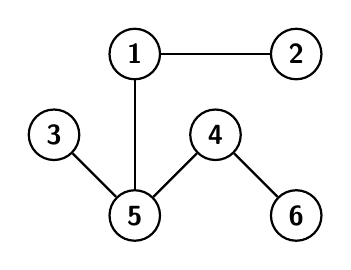
\begin{tikzpicture}[
    node distance=1.45cm, thick,
    main node/.style={circle, draw, font=\sffamily\bfseries}
]
    \node[main node] (1)                    {1};
    \node[main node] (3) [below left  of=1] {3};
    \node[main node] (4) [below right of=1] {4};
    \node[main node] (2) [above right of=4] {2};
    \node[main node] (5) [below right of=3] {5};
    \node[main node] (6) [below right of=4] {6};

    \path (1) edge (2)
        (1) edge (5)
        (3) edge (5)
        (4) edge (5)
        (4) edge (6);
\end{tikzpicture}
\caption{Et tre}
\end{figure}
 \end{column}
    \begin{column}{0.48\textwidth}
\begin{figure}
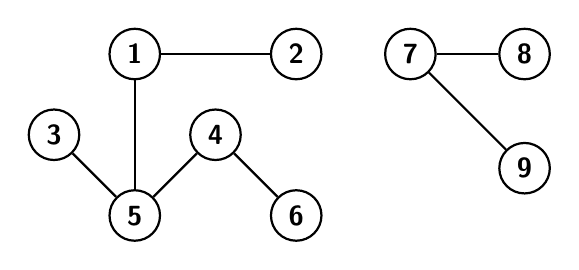
\begin{tikzpicture}[
    node distance=1.45cm, thick,
    main node/.style={circle, draw, font=\sffamily\bfseries}
]
    \node[main node] (1)                    {1};
    \node[main node] (3) [below left  of=1] {3};
    \node[main node] (4) [below right of=1] {4};
    \node[main node] (2) [above right of=4] {2};
    \node[main node] (5) [below right of=3] {5};
    \node[main node] (6) [below right of=4] {6};
    \node[main node] (7) [right of=2] {7};
    \node[main node] (8) [right of=7] {8};
    \node[main node] (9) [below of=8] {9};

    \path (1) edge (2)
        (1) edge (5)
        (3) edge (5)
        (4) edge (5)
        (4) edge (6)
        (7) edge (8)
        (7) edge (9);
\end{tikzpicture}
\caption{En skog (forest)}
\end{figure}
\end{column}
\end{columns}
\end{frame}

\begin{frame}{Rooted trees}
    \begin{block}{binary (m-ary) tre $G(V,E)$}
    Et tre med en root node der alle interne noder har eksakt to (m) barn.
    \end{block}
    \begin{columns}
    \begin{column}{0.48\textwidth}
\begin{figure}
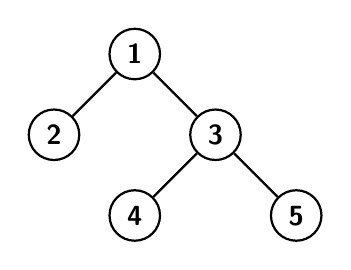
\begin{tikzpicture}[
    node distance=1.45cm, thick,
    main node/.style={circle, draw, font=\sffamily\bfseries}
]
   \node[main node] (1)                    {1};
    \node[main node] (2) [below left  of=1] {2};
    \node[main node] (3) [below right of=1] {3};
    \node[main node] (4) [below left of=3] {4};
    \node[main node] (5) [below right of=3] {5};

    \path (1) edge (2)
        (1) edge (3)
        (3) edge (4)
        (3) edge (5);
\end{tikzpicture}
\caption{binary tre}
\end{figure}
 \end{column}
    \begin{column}{0.48\textwidth}
\begin{figure}
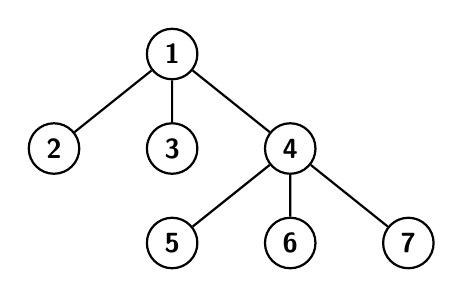
\begin{tikzpicture}[
    node distance=1.45cm, thick,
    main node/.style={circle, draw, font=\sffamily\bfseries},level distance=1.2cm,
  level 1/.style={sibling distance=1.5cm},
  level 2/.style={sibling distance=1.5cm}
]
  \node[main node] {1}
  	child {node[main node] {2}}
    child {node[main node] {3}}
    child {node[main node] {4}
    child {node[main node] {5}}
      child {node[main node] {6}}
    child {node[main node] {7}}
    };
\end{tikzpicture}
\caption{3-ary tre}
\end{figure}
\end{column}
\end{columns}
\end{frame}

\begin{frame}{Egenskaper}
    \begin{itemize}
        \item Et tre med $n$ noder har $n-1$ kanter
    \end{itemize}
   \begin{table}
    \begin{tabular}{l|l|l}
Noder & Interne noder & Leaves \\ \hline
\textbf{$n$} & $i=(n-1)/m$ & $l=((m-1)\cdot n+1)/m$\\
$n=m\cdot i + 1$ & \textbf{$i$} & $l=(m-1)\cdot i+1$\\
$n=(m\cdot l - 1)/(m-1)$ & $i=(l-1)/(m-1)$ & \textbf{$l$}          
\end{tabular}
\caption{Regne ut antall noder for fulle m-any trær}
\end{table}
\end{frame}

\begin{frame}{Eksempel}
Et kjedebrev starter med en person som sender et brev til fem andre mennesker. Hver person som får et brev sender den enten videre til fem andre eller stopper å sende ting videre.\\
Gå ut ifra at 10.000 personer sender brevet videre og ingen får brevet to ganger.\\
(1) Hvor mange personer fikk et brev?\\
(2) Hvor mange sendte ikke brevet videre?\\\pause
\begin{itemize}
\item Folk som sender videre: Interne noder $i=10000$
\item Folk som ikke sender videre: Leaves $l = (5-1)\cdot 10000 + 1 = 40001$
\item Folk som fikk et brev: Noder $n=5\cdot 10000 + 1 = 50001$
\end{itemize}
\end{frame}

\subsection*{Spørretid}
\begin{frame}{Spørsmål?}
    \begin{figure}
        \centering
        \includegraphics[height = 4.9cm]{images/guillaume9.jpg}
        \caption{Guillaume foran Tvindefossen}
        \label{fig:guillaume9}
    \end{figure}
\end{frame}
